\documentclass{article}
\usepackage[icelandic]{babel}
\usepackage[T1]{fontenc}
\usepackage[utf8]{inputenc}


\usepackage{subfig}

\usepackage{todonotes}
\usepackage{color}

%Leitað er af myndum í eftirfarandi möppum
\graphicspath{{./technical/}{./sprettir/}}
\linespread{1.5}
\setcounter{tocdepth}{2}

\usepackage{graphicx}
\usepackage{wrapfig}
\usepackage{float}
\usepackage{verbatim}
\usepackage[none]{hyphenat}





\begin{document}

\tableofcontents
\newpage

\section{Inngangur}
Skýrlsa þessi er um lokaverkefniverkefni í Tölvunarfræði við Háskólann í
Reykjavík, 
sem unnið var í samvinnu við DataMarket.

Verkefnið snérist um að búa til kerfi sem greinir
breytingar á tímalínum í gagnasafni Datamarket, 
sem gætu bent til þess að um markverða eða áhugaverða þróun sé að ræða.

Í skýrslunni er náin lýsing á verkefninu og hvernig vekráætlun var háttað.
Einnig greinum við frá þeim reikniaðferðum sem skoðaðar voru með tilliti til 	
\todo{stendur greinum 2x}
lausnar verkefnisins og greinum frá niðurstöðum okkar. Þá 
verður farið yfir atriði sem skoða mætti við nánari þróun kerfisins.
Að lokum er yfirlit yfir framvindu verksins.

\newpage
\section{Lýsing verkefnis}
Datamarket er fyrirtæki sem tekur sama töluleg gögn frá opinberum
stofnunum og einkaaðilum, gerir þau aðgengileg á einum stað og birtir þau á
auðskiljanlegan máta. Frá og með 25. janúar 2011 samanstóð gagnasafn þeirra 
af meira en 13.000 gagnasettum sem innihélt næstum 100 milljón tímalínur og 
fer það ört vaxandi.


Hvert gagnasett hjá DataMarket inniheldur tímaraðir sem sýna þróun tölulegra
stærða yfir tíma. 
Á hverjum degi eru tugir, eða jafnvel hundruð slíkra gagnasetta uppfærð í
kerfinu. 
Hvert gagnasett inniheldur að lágmarki eina, en allt að nokkurþúsund tímaraðir.
Sú		\todo{nokkurþúsund, tvo orð?}
þróun sem ein tímaröð sýnir getur verið allt frá vel
þekktum stærðum, s.s. verðbólgu, atvinnuleysi eða
hitastigi í Reykjavík, til mjög sérhæfðra eða jafnvel
undarlegra hluta, eins og innflutningsverðmæti
leðurvara frá Brasilíu!

Mikið er fylgst með algengustu stærðum og
stórvægilegar breytingar í þeim rata iðulega í fréttir	
umsvifalaust. En mjög markverð, áhugaverð eða jafnvel
varasöm þróun getur líka birst í stærðum sem fáir		\todo{er rett að
tala um stærðir, gögn?}
fylgjast með og enginn tekur etv. eftir. 

Þar sem óhagkvæmt er að fara handvirkt í gegnum þetta mikið magn af gögnum, 
til að finna áhugaverða atburði, var þörf á sjálfvirku kerfi til að 
sinna því hlutverki og fólst verkefni okkar í að útfæra það.

Upprunalega var kerfið hugsað á þann veg að það myndi athuga hvort ný gögn sem
væri verið að bæta við tímalínur Datamarket væru áhugaverð eður ei. Hinsvegar
varð ljóst í þróunnarferlinu að kerfið okkar gæti gert meira en unnið
eingöngu með nýjustu uppfærslurnar og varð því kerfið okkar yfirgripsmeira en
upprunalega stóð til.

Óskir Datamarket voru að fyrst yrði útbúið einfalt kerfi 
sem myndi greina meira en minna af áhugaverðum gögnum, jafnvel þó það myndi
mögulega 
innihalda mikið af ómarktækum niðurstöðum (e. false positives). Það var hugsað
sem 
grunnur sem hægt væri að byggja á. Því næst átti að þróa og greina aðferðir við
að 
bæta niðurstöðurnar. 

Fyrirhugað er að kerfið verði keyrt innan kerfis Datamarket.
\newpage

\section{Verkskipulag}

\subsection{Tímaskipulag}

Eitt af því fyrsta sem við gerðum þegar við byrjuðum að vinna að verkefninu var
að ákveða hvenær vikunar við myndum vinna að verkefninu. Þetta var mjög
mikilvægt vegna þess að meðlimir hópsins voru í ýmsum áföngum í skólanum, einnig
voru þrír af fjórum meðlimum hópsins dæmatíma kennarar í skólanum stóran hluta
verkefnistímans. 
Viku skipulagið leit svona út:

\vspace{5 mm}
\begin{tabular}{| l | l |}
\hline
  mánudagar & 12 - 3 \\
  \hline
  Þriðjudagar & 9 - 17 \\
  \hline
  Miðvikudagar & ekkert unnið sökum anna \\
  \hline
  Fimmtudagar & 12 - 4 \\
  \hline
  Föstudagar & 9 - 12\\
\hline
\end{tabular}
\vspace{5 mm}

Farið var eftir þessu skipulagi á meðan kennsla stóð yfir í skólanum alls átta
vikur (frá 30. janúar til 28. mars). 18 tímar í viku, alls 144 tímar á mann
miðað við átta vikum.
Eftir þessar átta vikur kom prófatími í háskólanum og lá því vinna í verkefninu
niðri. 
Að loknum prófum voru þrjár vikur sem meðlimir hópsins gátu einbeitt sér alfarið
að verkefninu. Sett var upp áætlun um að vinna í átta tíma á dag, sjö daga
vikunnar. Gerðum við því ráð fyrir að vinna 168 tíma á mann. 
Samtals hljómaði áætlunin uppá 312 tíma fyrir hvern meðlim hópsins. Inni í
áætluninn voru ekki tímarnir sem voru settir í undirbúning verkefnisins, þ.e.
þegar við vorum að funda með Hjálmari Gíslasyni hjá Datamarket og að setja saman
lýsingu verkefnisins haustið 2010.

\subsection{Aðferðafræði}

Við áttuðum okkur á því strax þegar við byrjuðum að skipuleggja okkur að þar sem
verkefnið fæli í sér töluverðar rannsóknir, þ.e. að finna út hvaða reiknirit og
reiknilíkön væru hentugust til að fá kerfið okkar til að virka eins og skildi
sem og prófanir á þeim, þá þyrftum við að hafa mikið og gott skipulag. Þetta
skipulag fengum við með því að notast Scrum aðferðafræðina þar sem að hún bíður
uppá að við gátum verið fljótir að bregðast við þegar e-ð var ekki að ganga sem
sem og tryggt að við færum ekki of langt frá upprunalega markmiði verkefnisins. 
Eins og kom fram að ofan þá byrjuðum við á því að útbúa einfalda frumgerð sem
gæfi okkur niðurstöður og síðan myndum við vinna í að betrumbæta það. Útfrá því
var verkefninu skipt upp í tvo fasa, fyrri fasinn var frumgerðarfasinn, sem stóð
yfir fyrstu átta vikurnar og síðan seinni fasann sem voru seinusta þrjár
vikurnar. Alls brutum við tímabilið niður í átta spretti, í fasa eitt voru fjóra
tveggja vikna sprettir, síðan settum við inn einn fjögra vikna sprett sem
innihélt prófvikurnar. Síðan var settur sprettur á hverja af seinustu þrem
vikunum.
Haldið var utan um alla skjölun s.s. kröfulista, framvindurit (e. burndown) og
dagbækur hópmeðlima. Notast var við Scrum vegg þar sem að sögur og verkefni
tengd þeim voru hengd upp til að fá yfirsýn yfir framvindu sprettanna. Gaf það
góða raun þar sem að það var ávalt í augsýn og hélt mönnum við efnið.

\subsection{Hlutverkaskipting}

Meðlimir hópsins tóku að sér hlutverk eins og mælt er með innan Scrum.
Hlutverkin voru eftirfarandi:

\vspace{5 mm}
\begin{tabular}{| l | l |}
\hline
Titill & Nafn \\
\hline
Scrum master & Þórður Bjarki Arnarson\\
\hline
Fulltrúi verkkaupa* & Arnór Barkarson \\
\hline
Forritarar & Allir \\
\hline
\end{tabular}
\vspace{5 mm}

*Taka ber fram að ástæðan fyrir þessum titili var að eiginlegur verkkaupi
verkefnisins var Hjálmar Gíslason ein þar sem að það þótti ekki ástæða fyrir
hann að vera taka beinan þátt í verkefninu, allavegana í fyrri fasa
verkefnisins, þá tók Arnór að sér að vera fulltrúi hans.



\newpage


\section{Rannsóknir}
\label{sec:research}
Til að kynna okkur mögulegar aðferðir sem gætu nýst við greiningu á gögnum
höfðum við samband við kennara og prófessora innan skólans. Henning Úlfarsson
varð fyrstur fyrir valinu og á fundi með honum kviknuðu flestar þær hugmyndir sem eru
í notkun í kerfinu í dag. Einnig áttum við fund með Bjarna Halldórssyni sem
kynnti fyrir okkur flóknari hugtök og benti okkur á ýmis hliðstæð verkefni.
Magnús Már Halldórsson og Sæmundur E. Þorsteinsson ráðlögðu okkur svo frekar í
öðrum reikniritum sem talað er um í Kafla 7.



\subsection{Bollinger bönd}
\label{sec:research_bollinger_bands}

Bollinger bönd eru upprunalega þróuð sem greiningartól
á þróun verðbréfaverða. 
Tilgangur þeirra er að veita viðeigandi skilgreiningu háum og lágum gildum.
Einnig hefur þessari 
aðferð verið beitt á ýmis önnur vandamál með misgóðum niðurstöðum. \\

Bollinger bönd samanstanda af:




\begin{itemize}
  \item Miðband, $N-lotu$ einfalt hlaupandi meðaltal\footnote[1]{Útskýringu á
hlaupandi meðaltali er að finna í tækniskýrslu á meðfylgjandi geisladisk.}.
  \item Efra band, $N-lotu$ staðalfrávik margfaldað með $K$, fyrir ofan
miðbandið ($HM + K\sigma$).
  \item Neðra band, $N-lotu$ staðalfrávik margfaldað með $K$, fyrir neðan
miðbandið ($HM -K\sigma$).
\end{itemize}







%\begin{wrapfigure}{r}{7cm}
\begin{figure}[H]
  \centering
  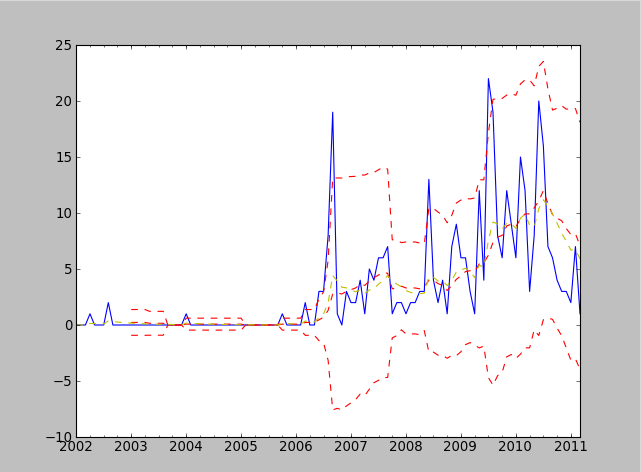
\includegraphics[width=.58\textwidth]{Bollinger.png} 
  \caption{Bollinger bönd merkt með Rauðum strikalínum} 
\end{figure}
%\end{wrapfigure}


Bollinger bönd nýtast því vel til greininga á því hvar í
tímalínu óeðlileg hækkun eða lækkun á sér stað.




\subsection{Fourier transformations} 

Fourier umbreytingar eru stærðfræðilegar aðgerðir

sem brjóta merki niður í tíðnir þess, hægt væri að umbreyta tímalínu í tíðnir. 
Ef ákveðin tíðni er mjög áberandi í tíðniritinu, þá er að öllum líkindum
endurtekning með þeirri tíðni í tímalínunni. 

Sem dæmi um slíkt er tímalínan á mynd~\ref{fig:rafmagnsnotkun} sem sýnir
rafmagnsnotkun í ótilgreindu landi.


\begin{figure}[H]
  \centering 
 
\subfloat[Tímalína]{\label{fig:rafmagnsnotkun}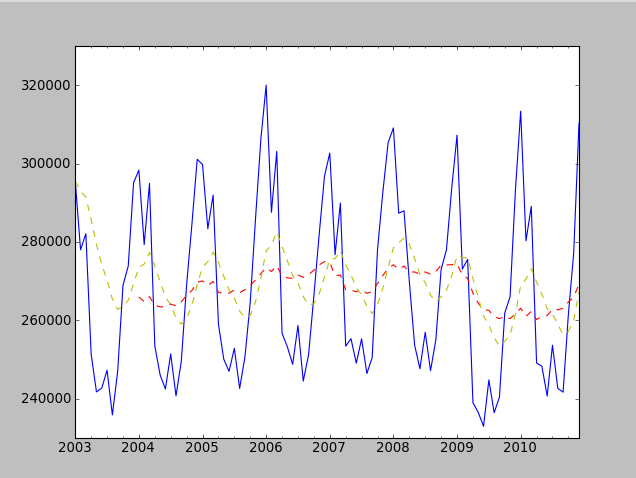
\includegraphics[width=0.42\textwidth]{Rafmagnsnotkun}}                    
 
\subfloat[Tíðnirit]{\label{fig:fouriergraph}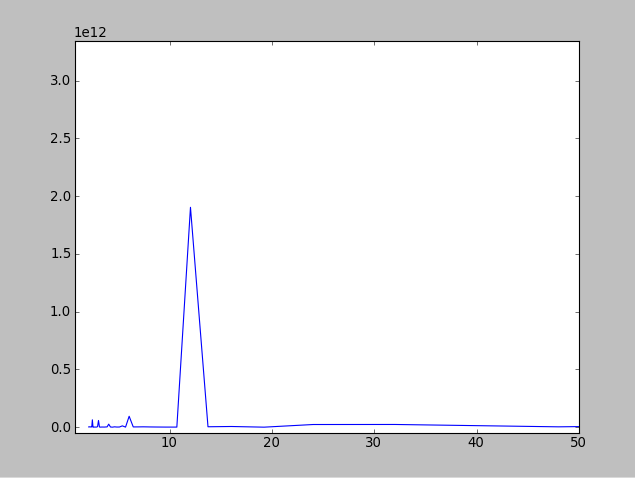
\includegraphics[width=0.42\textwidth]{Fourier}} 
  \caption{Fourier Transformations}
  \label{fig:fourier}
\end{figure}

Það má sjá að tímalínan hefur ákveðnar endurtekningar,

nánar tiltekið þá er mikil notkun á veturna en lítil á sumrin.
Þessa föstu sveiflu í tímalínunni greinir Fourier og skilar grafi á mynd~\ref{fig:fouriergraph}. 

Úr því er síðan hægt að greina að endurtekning á sér stað með 12 staka
millibili.

\subsection{Niðurstaða rannsókna}
Á vissum tímapunkti í verkefninu varð okkur ljóst að Bollinger bönd hentuðu
mjög vel fyrir mest af því sem við óskuðum að kerfið skyldi gera.
Því var sett aukin áhersla á að prófa mismunandi útfærslur Bollinger banda og
dregið úr prófunum annarra aðferða.

Hinsvegar eru annmarkar á þessari aðferð.

Sem dæmi má nefna línur sem innihalda mikinn fjölda punkta.
Líta má á þær tímalínur af \ilqq hærri\irqq \hspace{1pt} upplausn en þær sem innihalda fáa punkta. Í
þeim getur kerfið okkar verið að flagga punkta sem vissulega eru mjög
áhugaverðir séu þeir skoðaðir í því samhengi sem kerfið okkar sér þá þ.e. innan
rammans. Sé ramminn lítill er hægt að bera það saman við að kerfið sé að skoða
tímalínuna úr lítilli fjarlægð. Aftur á móti sé sama tímalína skoðuð úr meiri
fjarlægð getur línan virst svo gott sem flöt og því í heildina ansi óáhugaverð.

Í öðru dæmi væri hægt að hugsa sér tímalínu sem hækkar töluvert upp í ákveðinn
hápunkt og taki svo að lækka aftur niður í fyrri gildi. Gerist þetta með nógu
litlum breytingum á milli punkta er ólíklegt að kerfið okkar sjái nokkuð
athugavert við þetta þó að mögulega hafi eitthvað merkilegt átt sér stað. 

Í þessum tilvikum þyrfti að skoða tímalínurnar í öðru samhengi: út frá því hvort
það eigi sér stað breyting í hinu almenna ferli tímalínunnar. Bollinger böndin
eru ekki mjög gagnleg til þess þar sem að útkoman byggir að miklu leiti á hvaða
rammastærð er notuð en við höfum ekki fundið neina aðferð sem gagnast við að
finna hentuga rammastærð út frá gögnum í tímalínunni.

Fjallað verður um aðferðir sem gagnast við að skoða þessa eiginleika í kafla~\ref{sec:future}

\section{Útfærsla}
\label{sec:imp_our}

Reikniritið í Rýni byggir grunn sinn á Bollinger böndum eins og áður hefur komið fram.
Þar sem erfitt eða ómögulegt reynist að áætla rammastærðir sjálfvirkt þá notast Rýnir við nokkrar mismunandi
rammastærðir og ítrar í gegnum þær. Hver ítrun gefur öllum punktum í tímalínu ákveðið meðaltals vægi, til að reikna
vægi punkts notum við okkar eigin útgáfu af formúlu sem kallast 
$\%b$\footnote[1]{Útskýringu á upprunalegu $\%b$ formúlunni er að finna í tækniskyrslu á meðfylgjandi geisladisk}. 
\\ \hfil
\\ \hfil
Okkar breytta útgáfa virkar sem svo:
\begin{itemize}
  \item Punktar innan bandanna fá einkunn á bilinu 0-1
  \item Punktar utan bandanna fá einkunn sem samsvarar hlutfallslegri fjarlægð frá meðaltali rammans, >1
\end{itemize}


Hér fyrir neðan er síðan formúlan okkar:


\begin{center}
  $\%b=\frac{abs((item - avg[index])}{(upperlim[index] - avg[index]))}$
\end{center}


Hver rammastærð leggur sína einkunn við það sem fyrir stendur, hlutfallslega
miðað við fjölda ítranna.

Þegar litlar breytingar í tímalínu áttu sér stað yfir langt tímabil áttu
Bollinger böndin til með að 
þrengjast í við mikið. Það gerði það að verkum að smávægilegar breytingar eftir
rólegt tímabil fengu
óeðlilega hátt gildi. Til að koma í veg fyrir það er bandbreiddin púnktsins
borin saman við meðalbandbreidd
tímalínunnar, ef bandbreidd púnktins er margfalt þrengri en meðalbandbreiddin þá
er púnktinum gefin lægri einkunn. 

Algengt er að ef tímalína rís eða fellur hratt, þá eru margir púnktar í röð
taldir áhugaverðir, sem er mjög eðlilegt.
Kerfið býður þó upp á þann möguleika að skila einungis áhugaverðasta púnktinum
úr röð samliggjandi púnkta.




\section{Rýnir}
\subsection{Flæðirit}
\label{sec:flow_chart}

\begin{figure}[H]
  \centering
  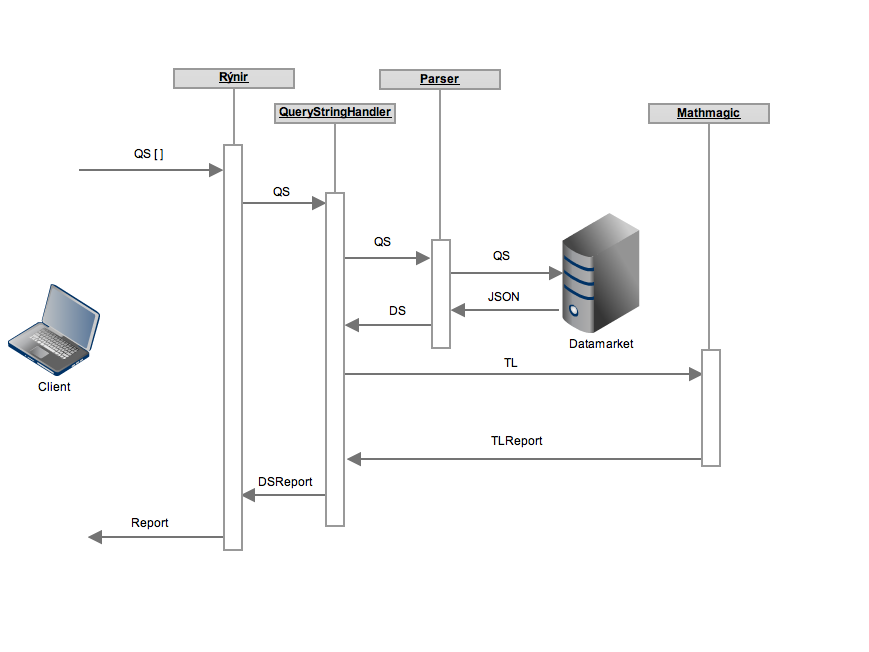
\includegraphics[width=.95\textwidth]{rynir_sequence-2.png} 
  \caption{Flæðirit} 
\end{figure}

Rýnir tekur við lista af fyrirspurnarstrengjum um gagnasett, sem táknað er með
QS[] á flæðiritinu, og skilar frá sér skýrslu um niðurstöðurnar fyrir öll
gagnasett úr listanum (Report). Hver fyrirspurnarstrengur (QS) í listanum er svo
réttur áfram til QueryStringHandlers, þessi virkni er þráðuð. Hver
QueryStringHandler sér svo um að láta Parser klasann sækja upplýsingar um
gagnasettið (JSON) í gagnagrunn DataMarket og skila til baka breyttu formi sem
hentar kerfinu (DS). Hver tímalína innan gagnasettsins er svo send til MathMagic
til greiningar sem skilar frá sér lista af flöggum fyrir tímalínuna (TLReport).
QueryStringHandler tekur saman niðurstöðurnar úr hverri tímalínu og skilar
sameinaðri niðurstöðu fyrir allt gagnasettið (DSReport).

Að neðan má svo sjá klasarit fyrir Rýnir

\begin{figure}[H]
  \centering
  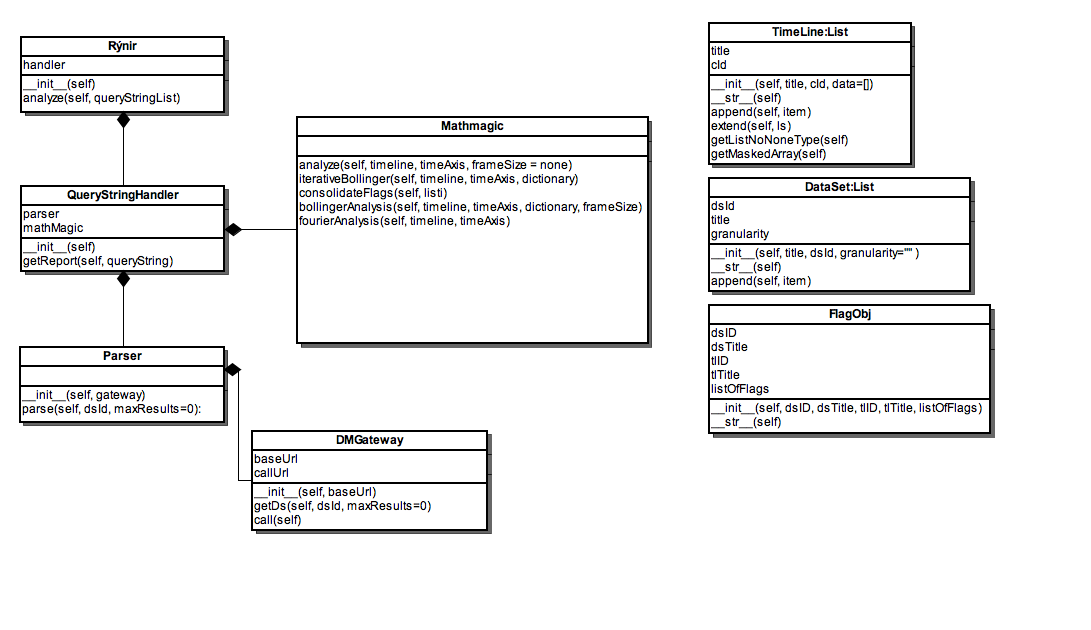
\includegraphics[width=.95\textwidth]{rynir_class_diagram.png} 
  \caption{Klasarit} 
\end{figure}

\section{Horft til framtíðar}
\label{sec:future}

\subsection{Linear Regression}
Í þessari aðferð má hugsa sér að reynt sé að draga eins fáar beinar línur í
gegnum almenna ferli tímalínunnar. Sé hægt að gera það með einni línu má líta
svo á að engin stórvægileg breyting eigi sér stað í almenna ferlinu og því í
heild sinni sé tímalínan óáhugaverð. Sé ekki hægt að gera það með einni línu
hefur átt sér stað nægileg breyting og má þá líta á skurðpunkt línanna sem
hugsanlega áhugaverðan punkt í tímalínunni.

\subsection{Fourier Transformation}
Eins og fjallað var um í kaflanum Rannsóknir nýtist Fourier
Transformation við að finna endurtekningar í tímalínum með því að brjóta þær
niður í tíðnir sínar.  
Einnig væri ekki einungis hægt að finna hvort það eigi sér stað endurtekning í
tímalínunni, heldur hvar. Þannig væri mögulegt að skoða endurtekningarnar nánar,
t.d. út frá því hvort ein endurtekningin sé óeðlilega há eða lág, eða hvort hana
hreinlega vanti eitt árið.




\section{Framvinda}
\subsection{Sprettir}
Verkefnið okkar var þannig lagt upp af DataMarket, að þeir vildu í fyrsta lagi
fá heilstætt kerfi sem skilaði niðurstöðum. 
Þær niðurstöður þyrftu þó ekki að vera mjög marktækar og byggja á flóknum
reikniaðferðum. Því næst áttum við að þróa reikniaðferðirnar eins 
mikið og mögulegt væri, á þeim tíma sem við höfðum. Þetta verkefni var því mjög
opið og ljóst að mikilvægt væri 
af okkar hálfu að halda góðri yfirsýn allan tímann, svo að ekki yrði farið
lengra í bætingum en svo að það myndi nást að fullklára þær 
aðferðir sem við ætluðum að hafa í kerfinu, í tæka tíð. Því lögðum við upp með
að vinna verkið í tveimur fösum. Áætlunin var þannig að skipuleggja
einungis fyrri fasan í upphafi. Byrja að kynna okkur meðfram þeim fasa hvað við
gætum mögulega gert í seinni fasanum, en taka ekki ákvarðanir 
um hvað yrði gert fyrr en í upphafi seinnifasa.

\subsubsection{Sprettur 0}
Sprettur 0 var settur upp sem undirbúnings sprettur. Ekki voru sögur eins og í
hefbundnum spretti, heldur notuðum við þennan tíma til að 
skipuleggja verkáætlun, gerðum áhættugreiningu og unnum að ýmsum öðrum
undirbúiningi.
\subsubsection{Sprettur 1}
Í fyrsta spretti fórum við í að kynna okkur tæknileg atriði sem við ætluðum að
nota.
Flest þekktum við, en höfðum ekki unnið með í Python áður. Þetta voru hlutir
eins og prófandrifin þróun, REST-ful þróun og hvernig 
unnið er með JSON skrár. Einnig settum við upp grunn að kerfinu sem gat sótt
gögn frá DataMarket. Náðum ekki alveg að kára það sem við lögðum 
upp með og urðum að færa hluta úr sögum yfir í næsta sprett.
\begin{figure}[H]
  \centering
  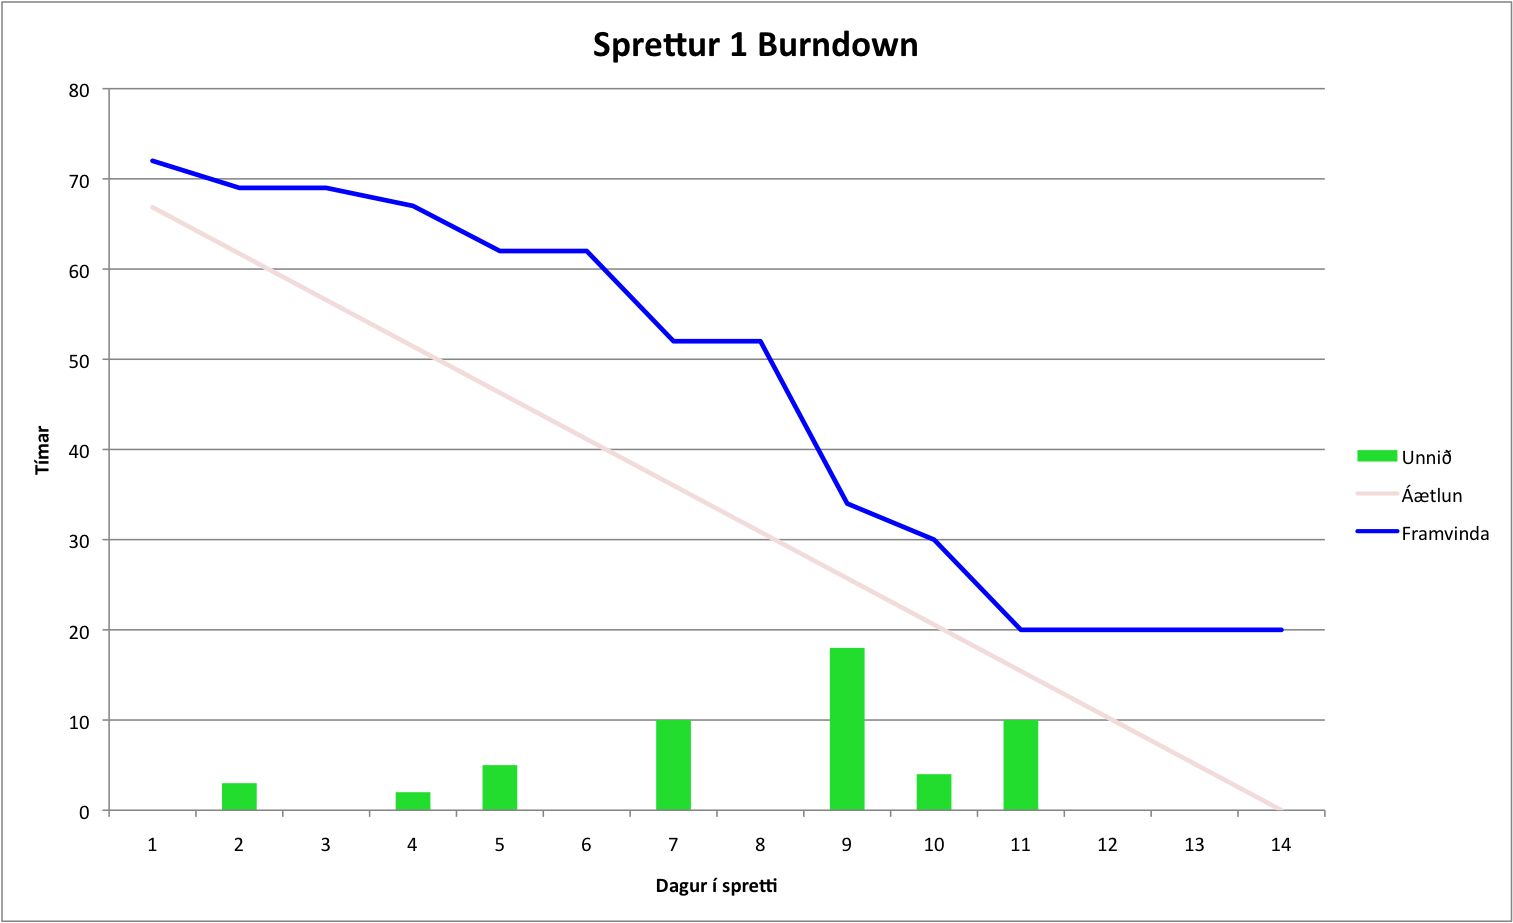
\includegraphics[width=0.72\textwidth]{Sprettur1_Burndown.png}
  \caption{Sprettur 1 Burndown}
\end{figure}

\subsubsection{Sprettur 2}
Í spretti 2 fundum við áhugaverð gögn hjá Datamarket settum upp staðbunda
gátt(e.service stub),svo að það myndi ekki hindra okkur í þróun ef 
aðgangur að gagnagrunni Datamarket væri ekki til staðar. Þetta var hluti af
okkar áhættugreiningu (VÍSUN í KAFLA). 
Þá bjugum við til fyrstu reikniaðferðirnar, meðaltal, miðgildi og staðalfrávik,
og létum kerfið sækja gögn og skila niðurstöðum.
Þá áttum við fundi með sérfræðingum á sviði stærðfræði og tölfræði, til að ýta
úr vör hugmyndavinnu fyrir seinni fasa.
\begin{figure}[H]
 \centering
 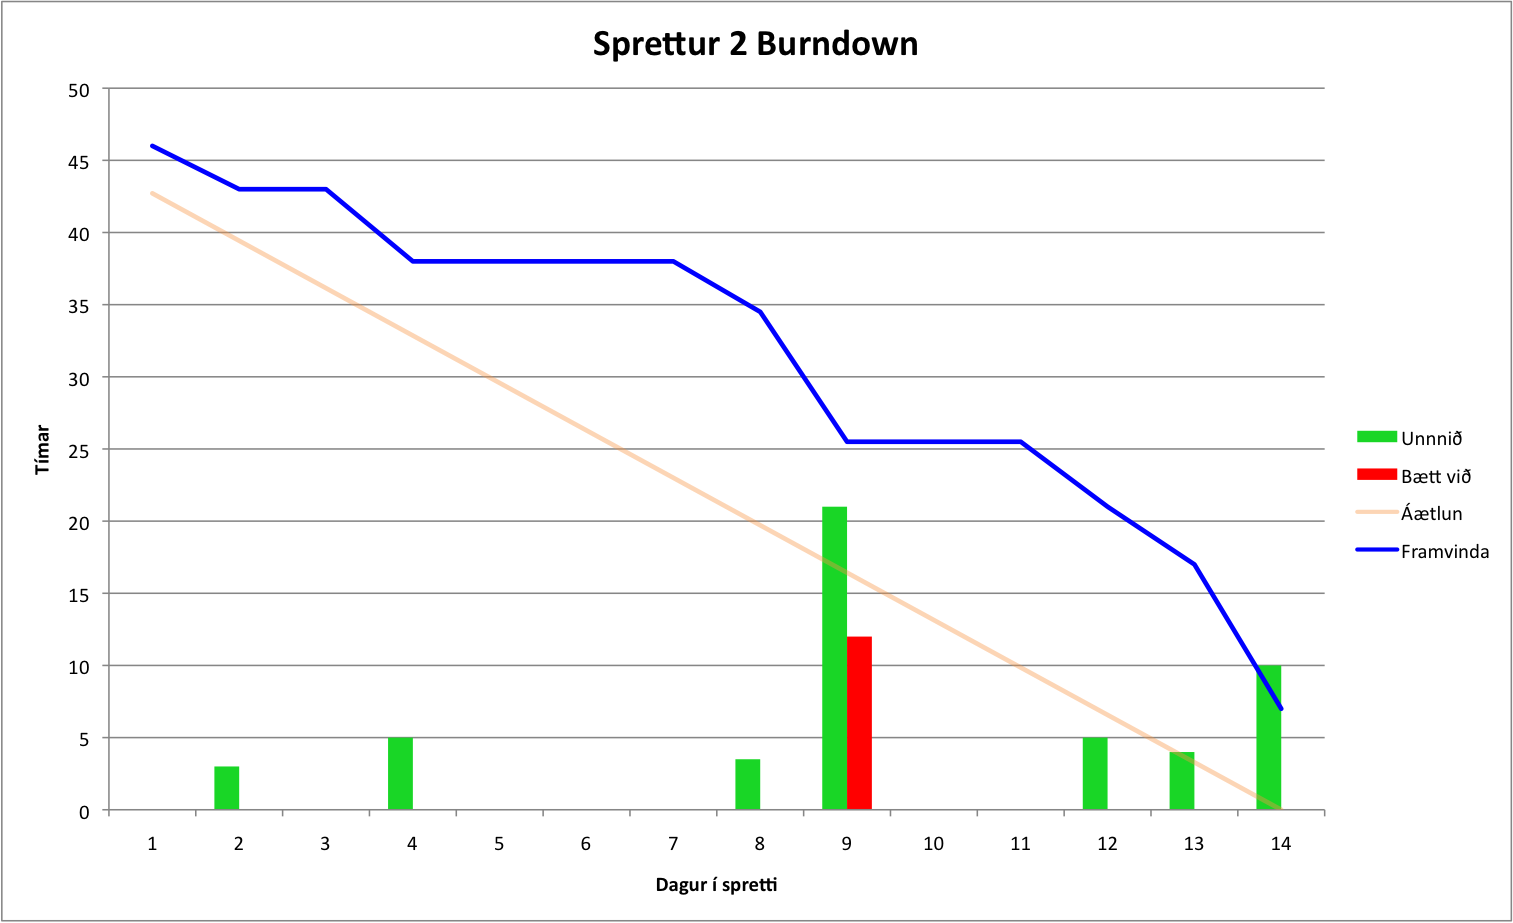
\includegraphics[width=0.72\textwidth]{Sprettur2_Burndown.png}
 \caption{Sprettur 2 Burndown}
\end{figure}
\subsubsection{Sprettur 3}
Þegar hér var komið við sögu vorum við farnir að finna ákveðinn takt í
áætlanagerð og sáum betur hvað við gátum gert ráð fyrir að klára mikið 
í einum sprett. Setum upp aðgerðarsöfn(e. libraries) sem voru til þess fallin að
aðstoða okkur við útreikninga. Það tók þó umtalsvert meiri tíma en við gerðum
ráð fyrir. Þá bættum við staðbundnu gáttina og kynntum okkur aðgerðarsöfnin.
\begin{figure}[H]
 \centering
 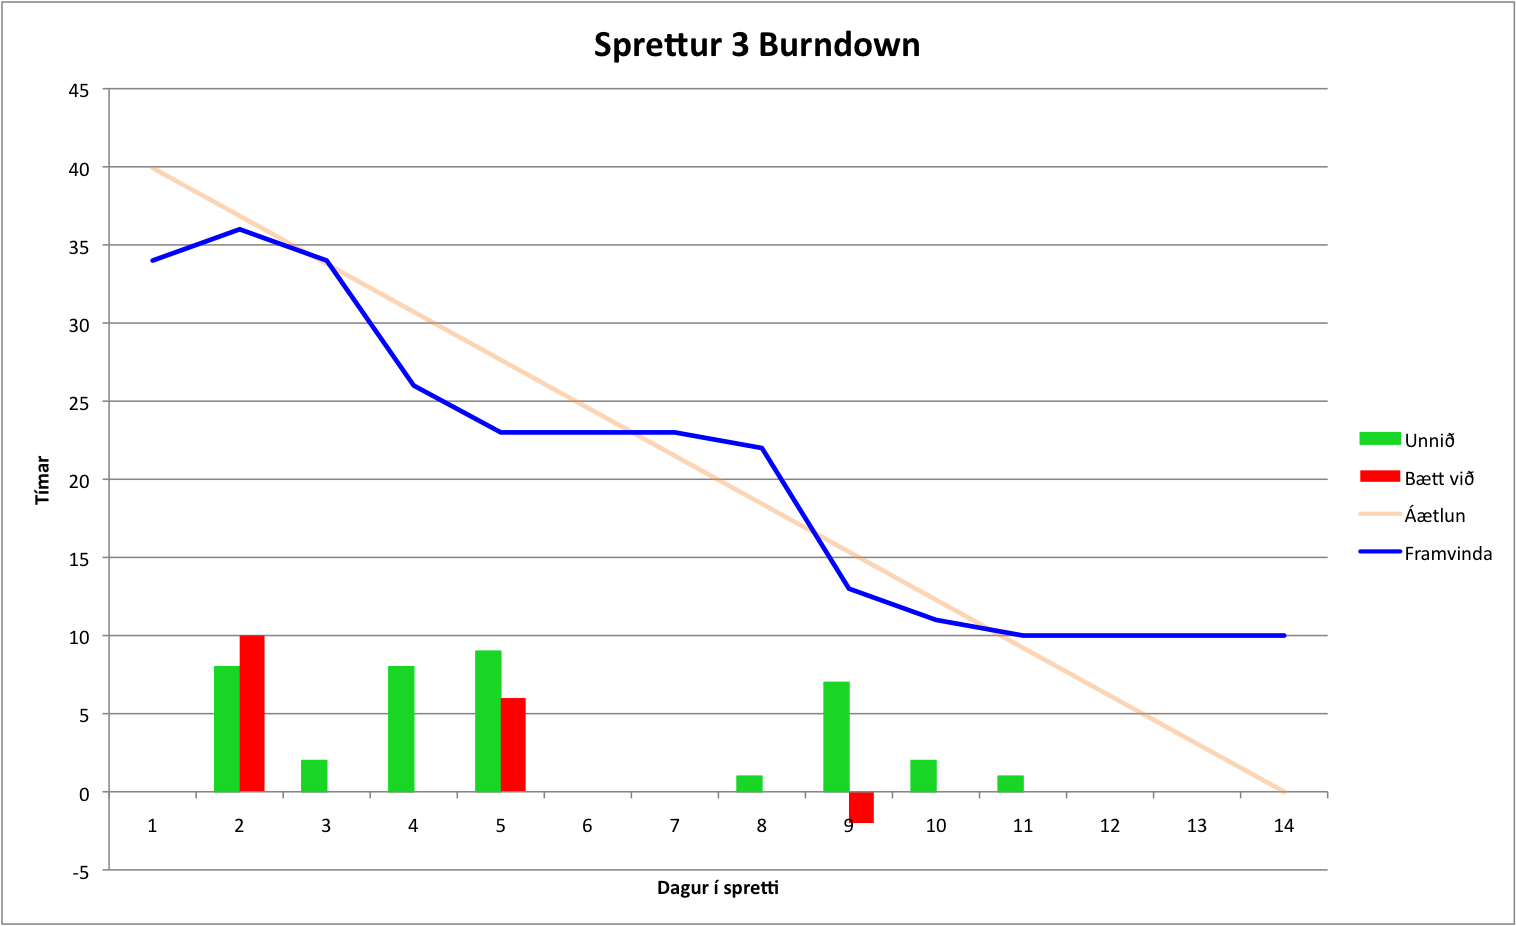
\includegraphics[width=0.72\textwidth]{Sprettur3_Burndown.png}
 \caption{Sprettur 3 Burndown}
\end{figure}
\subsubsection{Sprettur 4}
Spretturinn fór í að setja upp framenda á kerfið og forma skýrsluna sem það
skilar af sér. Þegar við vorum svo farnir að nota aðgerðarsöfnin 
kom á daginn að einföldu aðferðirnar okkar voru mun betri en vonir stóðu til.
Einnig komumst við að því að það hafa aðrir beitt þessum aðferðum 
og kallast þær Bollinger bönd ( SJÁ KAFLA UM BOLLINGER BÖND ). 

Við gátum nú sýnt þeim hjá Datamarket niðurstöður úr kerfinu okkar og við það
urðu til fleiri hugmyndir um hvernig hægt væri að nýta það ( SJÁ LÝSING
VERKEFNIS ).

Við skipulögðun sprettinn létt og kláruðum snemma þar sem próf voru framundan.
\begin{figure}[H]
 \centering
 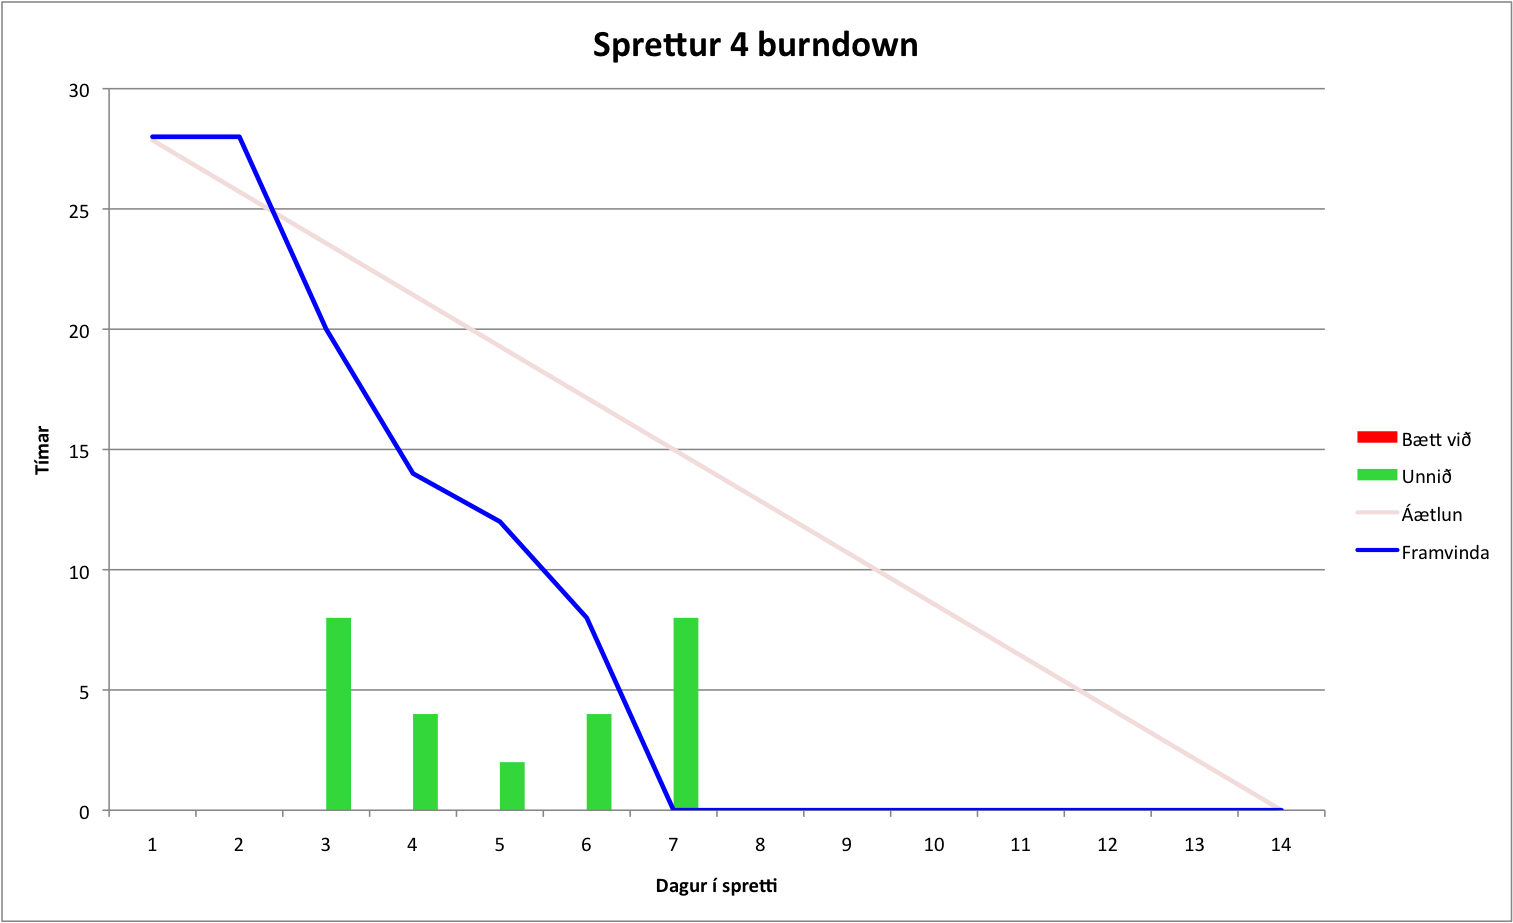
\includegraphics[width=0.72\textwidth]{Sprettur4_Burndown.png}
 \caption{Sprettur 4 Burndown}
\end{figure}

\subsubsection{Sprettur 5}
Síðasti sprettur í fasa 1. Funduðum með DataMarket og ákváðum endanlegt form á
flöggum sem er skilað. Gengum frá lausum endum, og kóði yfirfarinn 
(e. refactor) og útgáfa 1.0 varð til. Hugmyndavinna fyrir fasa 2 komin á fullt.

\begin{figure}[H]
 \centering
 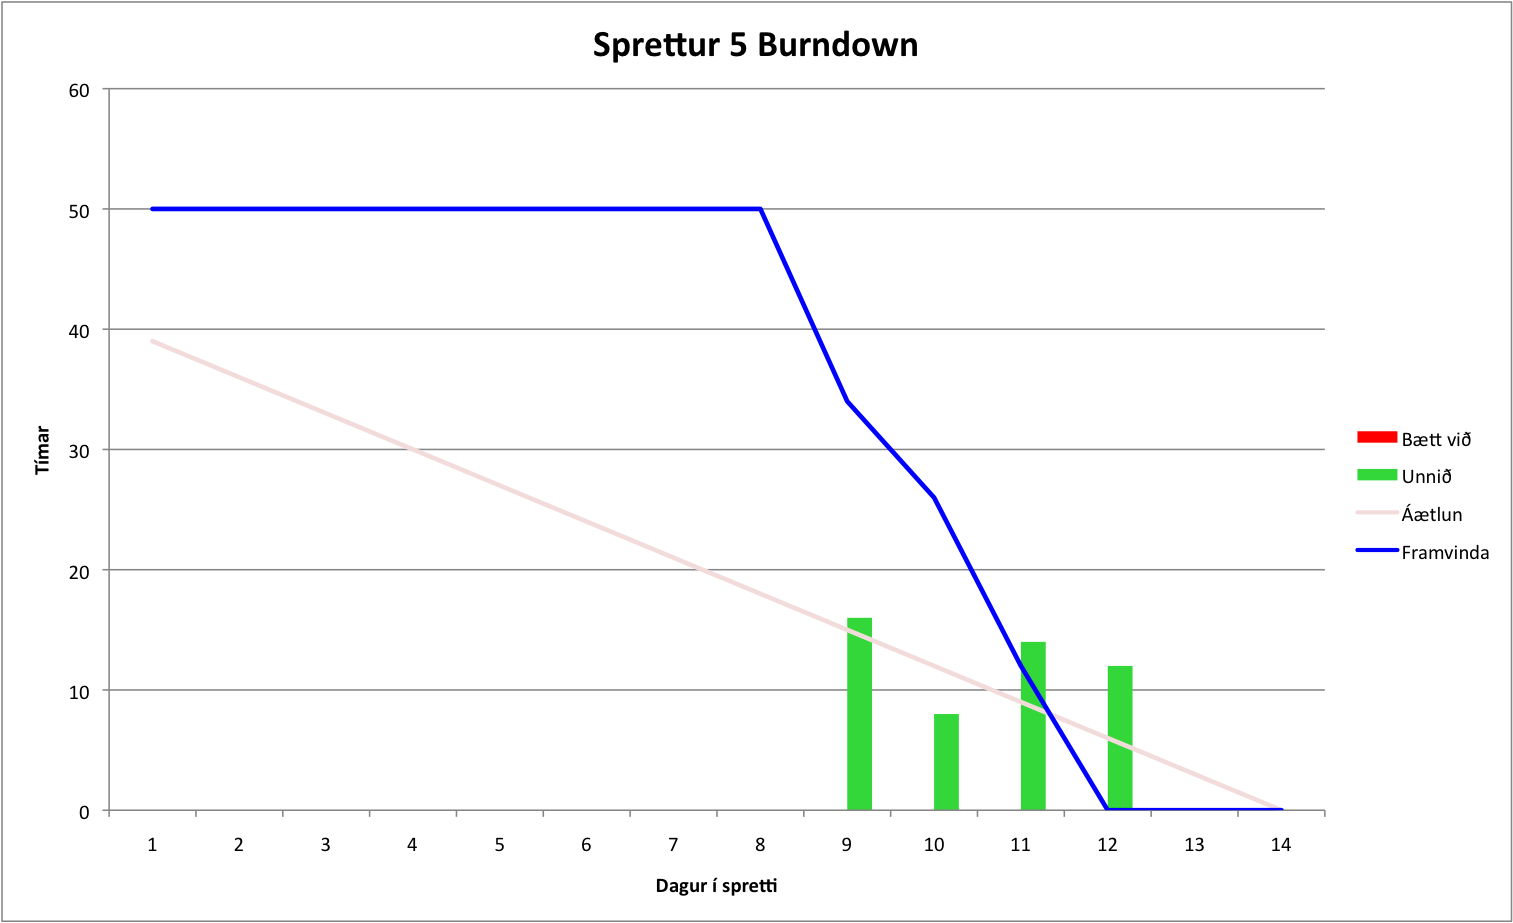
\includegraphics[width=0.72\textwidth]{Sprettur5_Burndown.png}
 \caption{Sprettur 5 Burndown}
\end{figure}

\subsubsection{Sprettur 6}
Við höfðum sankað að okkur mikið af upplýsingum og höfðum ákveðnar hugmyndir um
hvað okkur langaði að gera. Það krafðist þess hinsvegar að við 
þurftum að framkvæma prófanir til að sjá hvað myndi henta okkar kerfi best. Því
skipulögðum við sprettinn létt og bættum í hann þegar líða tók á. 
Fljótlega komumst við þó að niðurstöðum um hvaða útfærslur við vildum nota ( SJÁ
TÆKNIKAFLA ). Vinna við lokaskýrslu hófst. Í lok sprettsins 
vorum við komnir með verulega bættar reikniaðgeðir frá því sem var.

\begin{figure}[H]
 \centering
 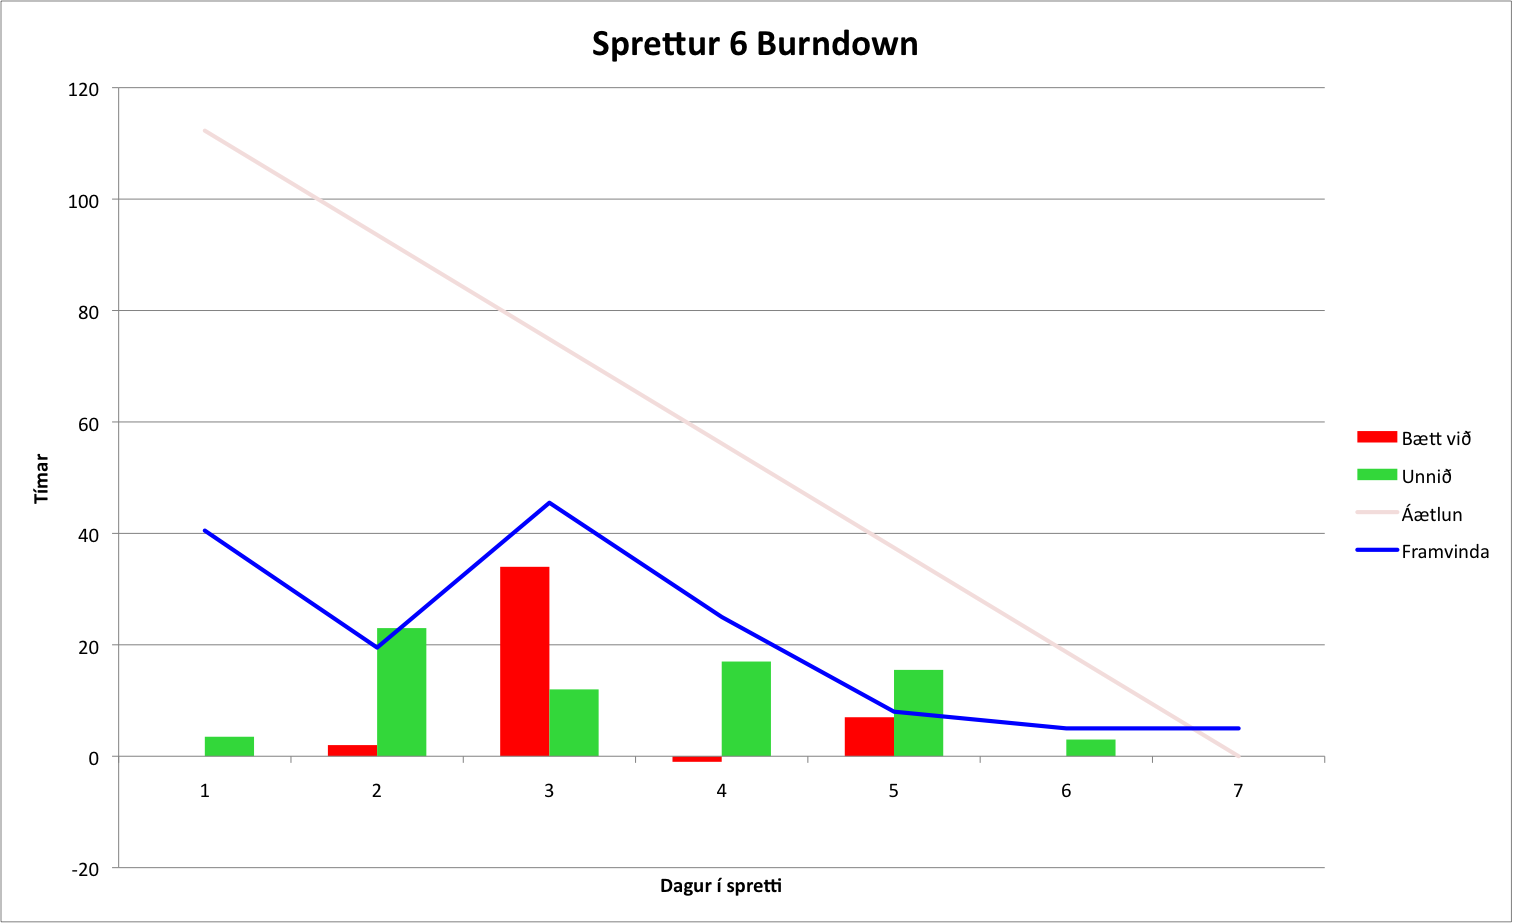
\includegraphics[width=0.72\textwidth]{Sprettur6_Burndown.png}
 \caption{Sprettur 6 Burndown}
\end{figure}

\subsubsection{Sprettur 7}
Byrjað á lokafrágangi. Allar keyrslustillingar lesnar úr skrá og villumeðhöndlun
yfirfarin. Sett upp log kerfi. Álagsprófanir framkvæmdar og 
niðurstöður úr þeim yfirfarnar. Fínstillingar á reikniritum í kjölfar prófanna
og villur lagfærðar. 

\begin{figure}[H]
 \centering
 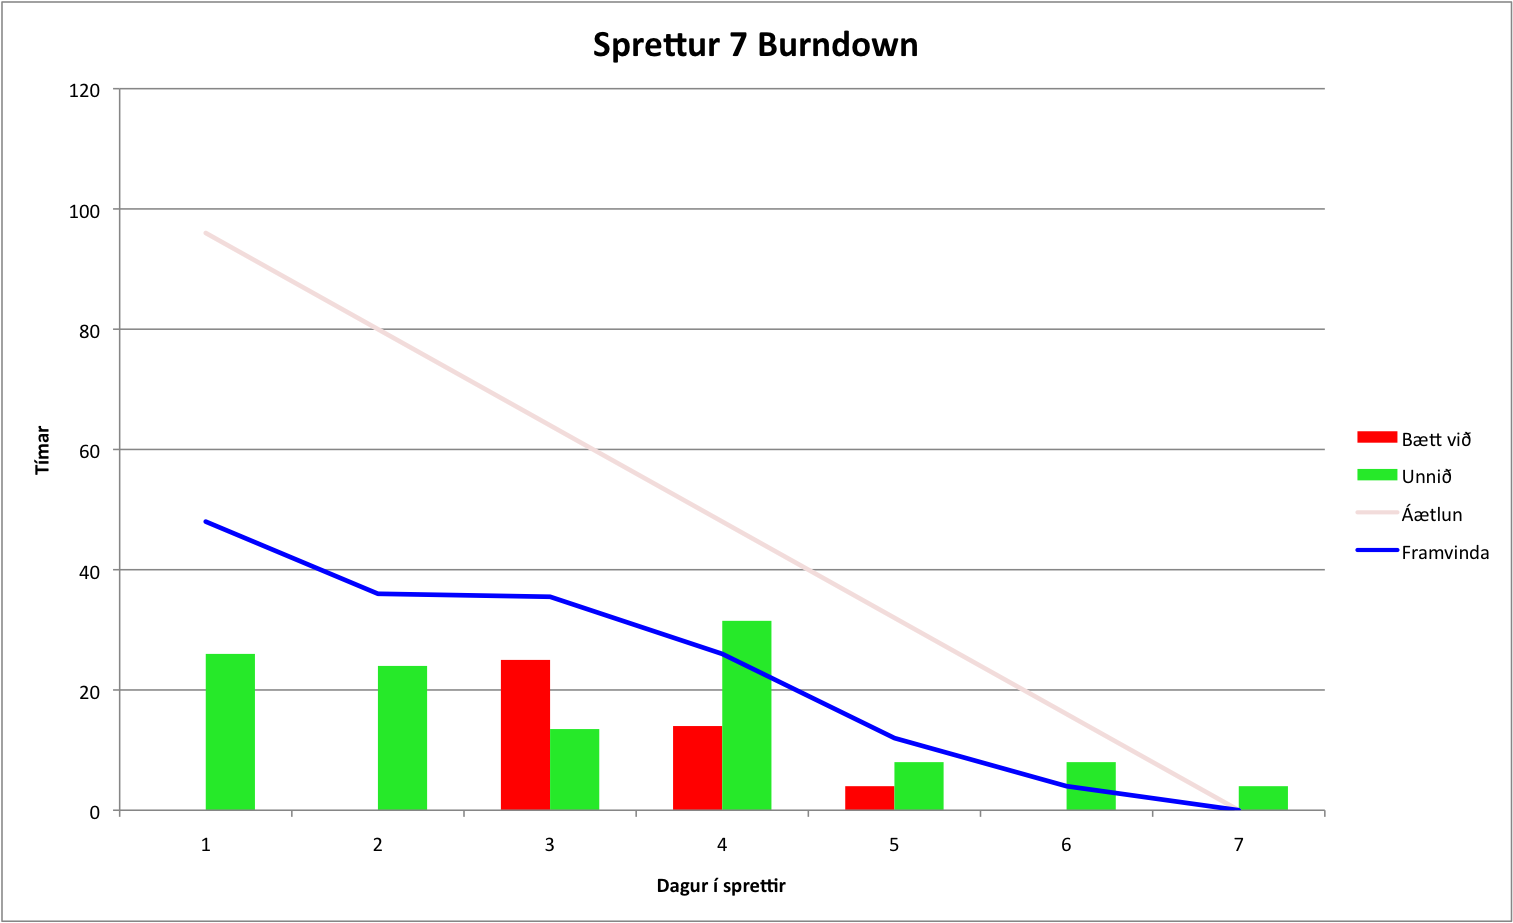
\includegraphics[width=0.72\textwidth]{Sprettur7_Burndown.png}
 \caption{Sprettur 7 Burndown}
\end{figure}

\subsubsection{Sprettur 8}
Skýrslugerð í aðalatriði í lokasprett. Lokafrágangur á kóða. Læddum inn einni
bætingu á reikniaðferðum og prófuðum uppá nýtt.
\begin{figure}[H]
 \centering
 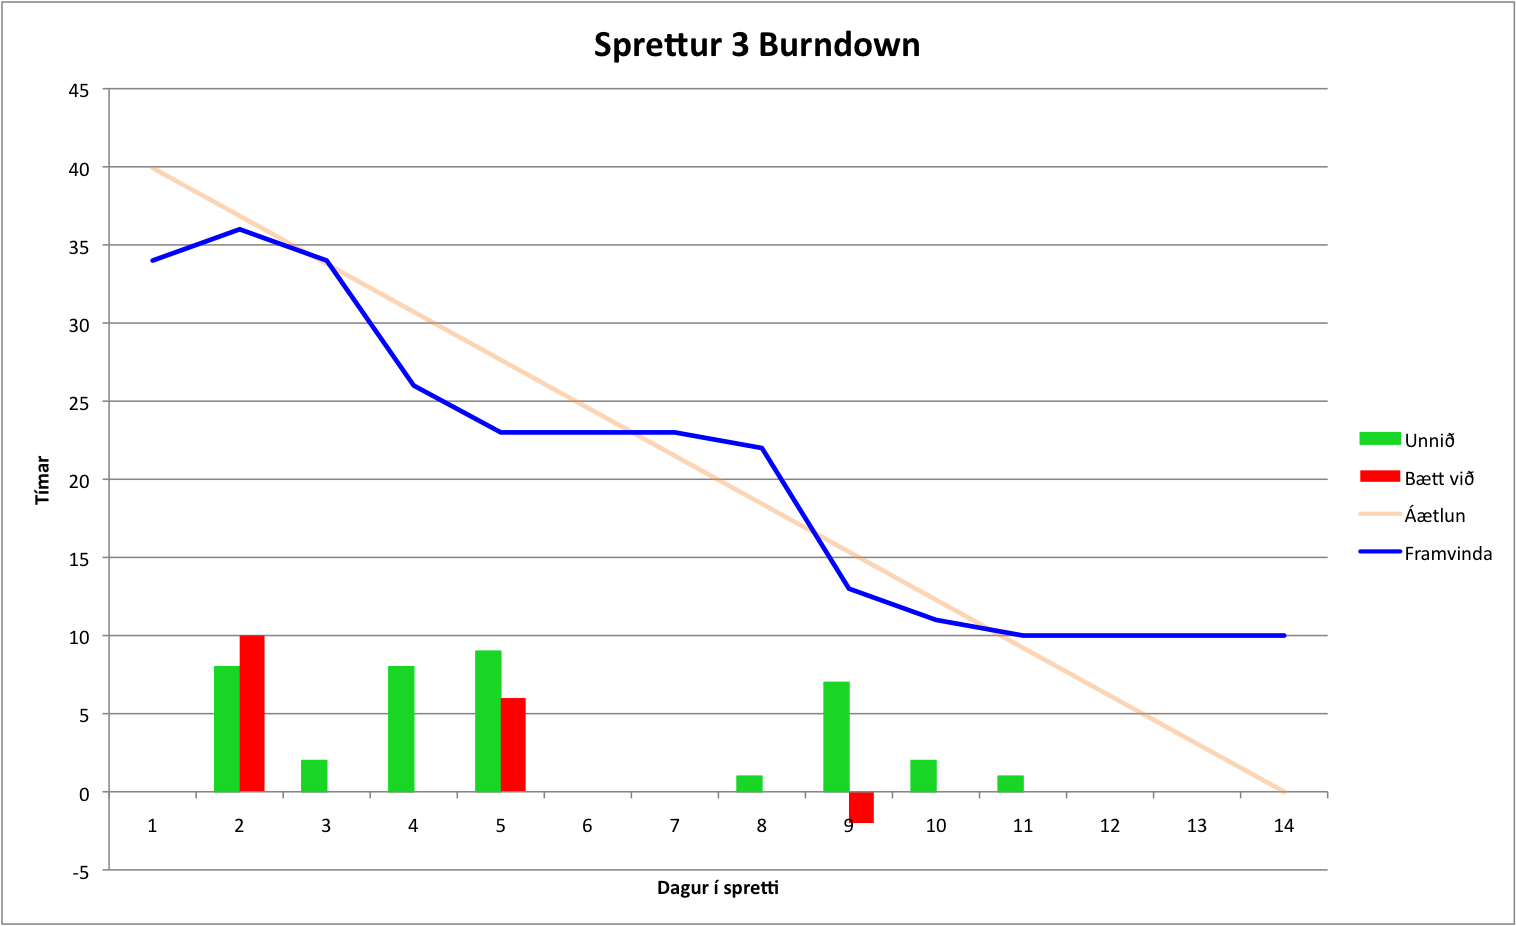
\includegraphics[width=0.72\textwidth]{Sprettur3_Burndown.png}
 \caption{Sprettur 8 Burndown RÖNG MYND}
\end{figure}

\hfil \\
\hfil \\
\hfil \\
\hfil \\

\end{document}